\documentclass[11pt, addpoints, answers]{exam}

\usepackage{amsmath, amssymb, euler}
\usepackage{xcolor}
\usepackage{algorithm, algorithmicx, algpseudocode}
\usepackage{tikz, tikz-qtree, drawstack}
\usepackage[shortlabels]{enumitem}

\usetikzlibrary{graphs}
\tikzset{every tree node/.style={minimum width=2em,draw,circle},
	blank/.style={draw=none},
	edge from parent/.style=
	{draw,edge from parent path={(\tikzparentnode) -- (\tikzchildnode)}},
	level distance=1.2cm}

% For inserting code snippets.
\usepackage{listings}
\lstset{
    columns = fixed,
    basewidth = {0.5em},
    breaklines = true,
    backgroundcolor = \color{white},
    keywordstyle = \color[RGB]{40, 40, 255},
    numberstyle = \footnotesize\color{darkgray},
    commentstyle = \ttfamily\color{violet},
    basicstyle = \ttfamily,
    stringstyle = \ttfamily\color[RGB]{128, 0, 0},
    showstringspaces = false,
    language = {[11]C++},
    escapechar = \@
}
\lstnewenvironment{cpp}[1][]{\lstset{language = {[11]C++}, #1}}{}

\usepackage{tikz}

% headers, footers, titles
\newcommand{\CourseName}{CS101 Algorithms and Data Structures}
\newcommand{\HomeworkNO}{Homework 4}
\newcommand{\DueDate}{Due date: 23:59, November 5th, 2023}

\pagestyle{headandfoot}
\runningheadrule
\runningheader{\CourseName}{\HomeworkNO}{\DueDate}
\runningfooter{}{\thepage}{}

\title{
	\CourseName\\
	Fall 2023\\
	\HomeworkNO
}
\author{}
\date{\DueDate}

% formats of questions, choices, points, etc.
\qformat{\bf\thequestion. (\totalpoints\ points) \thequestiontitle\hfill}
\pointname{'}
\CorrectChoiceEmphasis{\bf\color{blue}}
\SolutionEmphasis{\color{blue}}

% We frequently use this font.
\newcommand{\ttt}{\texttt}

\begin{document}

\maketitle

\begin{enumerate}
	\item Please write your solutions in English.
	\item Submit your solutions to gradescope.com.
	\item Set your FULL name to your Chinese name and your STUDENT ID correctly in Account Settings.
	\item If you want to submit a handwritten version, scan it clearly. \ttt{CamScanner} is recommended.
	\item When submitting, match your solutions to the problems correctly.
	\item No late submission will be accepted.
	\item Violations to any of the above may result in zero points.
\end{enumerate}

\newpage

{\large\textbf{Notes}:}

\begin{enumerate}
	\item Some problems in this homework requires you to design divide-and-conquer algorithm. When grading these problems, we will put more emphasis on how you reduce a problem to a smaller size problem and how to combine their solutions with divide-and-conquer strategy. 
	\item Your answer for these problems {\color{red}\textbf{should}} include:
	\begin{enumerate}
		\item {\color{red} \textbf{Clear description} of your algorithm design in \textbf{natural language}, with \textbf{pseudocode} if necessary.}
		\item {\color{red}Run-time Complexity Analysis}
            \item {Proof of Correctness (If required)}
	\end{enumerate}
    \item Your answer for these problems is {\color{red}not allowed to include real C or C++ code}.
	\item In your description of algorithm design, you should describe each step of your algorithm clearly.
	\item You are encouraged to write pseudocode to facilitate explaining your algorithm desgin, though this is not mandatory. If you choose to write pseudocode, please give some additional descriptions to make your pseudocode intelligible.
	\item You are recommended to finish the algorithm design part of this homework with \LaTeX.
\end{enumerate}

\begin{questions}

\titledquestion{Binary Search Example}[0]

Given a sorted array $a$ of $n$ elements, design an algorithm to search for the index of given element $x$ in $a$.

\begin{solution}


\textbf{Algorithm Design:} We basically ignore half of the elements just after one comparison.
\begin{enumerate}
	\item Compare $x$ with the middle element.
	\item If $x$ matches with the middle element, return the middle index.
	\item Else If $x$ is greater than the mid element, then $x$ can only lie in right half subarray after the mid element. So we recur for right half.
	\item Otherwise ($x$ is smaller) recur for the left half.
\end{enumerate}

\textbf{Pseudocode(Optional):}\\
$left$ and $right$ are indices of the leftmost and rightmost elements in given array $a$ respectively.
\begin{algorithm}[H]
    \color{blue}
	\begin{algorithmic}[1]
		\Function {binarySearch}{a, value, left, right}
		\If {right $<$ left} 
		\State \Return not found
		\EndIf
		\State mid $\gets \lfloor (right-left)/2 \rfloor + left$
		\If {a[mid] = value} 
		\State \Return mid
		\EndIf
		\If {value $<$ a[mid]} 
		\State \Return binarySearch(a, value, left, mid-1)
		\Else
		\State \Return binarySearch(a, value, mid+1, right) 
		\EndIf   		
		\EndFunction
	\end{algorithmic}
\end{algorithm}

\textbf{Proof of Correctness:}
If $x$ happens to be the middle element, we will find it in the first step. Otherwise, if $x$ is greater than the middle element, then all the element in the left half subarray is less than $x$ since the original array has already been sorted, so we just need to look for $x$ in the right half subarray. Similarly, if $x$ is less than the middle element, then all the element in the right subarray is greater than $x$, so we just need to look for $x$ in the front list. If we still can't find $x$ in a recursive call where $left = right$, which indicates that $x$ is not in $a$, we will return $not\; found$ in the next recursive call.

\textbf{Time Complexity Analysis:}
During each recursion, the calculation of $mid$ and comparison can be done in constant time, which is $O(1)$. We ignore half of the elements after each comparison, thus we need $O(\log n)$ recursions.
$$T(n) = T(n/2)+O(1)$$\\
Therefore, by the Master Theorem $\log_{b}{a}=0=d$, so $T(n) = O(\log n)$.

\end{solution}

\newpage

\titledquestion{Multiple Choices}

Each question has \textbf{one or more} correct answer(s). Select all the correct answer(s). For each question, you will get 0 points if you select one or more wrong answers, but you will get 1 point if you select a non-empty subset of the correct answers.

Write your answers in the following table.

\begin{table}[htbp]
    \centering
    \begin{tabular}{|p{2cm}|p{2cm}|p{2cm}|p{2cm}|}
        \hline
        (a) & (b) & (c) \\
        \hline
        %%%%%%%%%%%%%%%%%%%%%%%%%%%%%%%%%%%%%%%%%%%%%%%%%%%%%%%%%%
        % YOUR ANSWER HERE.
          AB  &  D   &  AC   \\
        %%%%%%%%%%%%%%%%%%%%%%%%%%%%%%%%%%%%%%%%%%%%%%%%%%%%%%%%%%
        \hline
    \end{tabular}
\end{table}

\begin{parts}
        
    \part[3] Which of the following sorting algorithms can be implemented as the stable ones?
    \begin{choices}
        \CorrectChoice  Insertion-Sort 
        \CorrectChoice Merge-Sort
        \choice Quick-Sort (always picking the first element as pivot)
        \choice None of the above
    \end{choices}
    
    \part[3] Which of the following implementations of quick-sort take \(\Theta(n\log n)\) time in the \textbf{worst case}?
    
    \begin{choices}
        \choice Randomized quick-sort, i.e. choose an element from \(\left\{a_l,\cdots,a_r\right\}\) randomly as the pivot when partitioning the subarray \(\langle a_l,\cdots,a_r\rangle\).
        \choice When partitioning the subarray \(\langle a_l,\cdots,a_r\rangle\) (assuming \(r-l\geqslant 2\)), choose the median of \(\left\{a_x,a_y,a_z\right\}\) as the pivot, where \(x,y,z\) are three different indices chosen randomly from \(\{l,l+1,\cdots,r\}\).
        \choice When partitioning the subarray \(\langle a_l,\cdots,a_r\rangle\) (assuming \(r-l\geqslant 2\)), we first calculate \(q = \frac{1}{2} (a_{\max} + a_{\min})\) where \(a_{\max}\) and \(a_{\min}\) are the maximum and minimum values in the current subarray respectively. Then we traverse the whole subarray to find \(a_m \; s.t. \left|a_m - q\right| = \min_{i=l}^r \left|a_i - q\right|\) and choose \(a_m\) as the pivot.
        \CorrectChoice None of the above.
    \end{choices}

    \part[3] Which of the following statements are true?
    
    \begin{choices}
        \CorrectChoice If \(T(n) = 2T(\frac{n}{2}) + O(\sqrt{n})\) with \(T(0) = 0\) and \(T(1) = 1\), then \(T(n) = \Theta(n)\).
        \choice If \(T(n) = 4T(\frac{n}{2}) + O(n^2)\) with \(T(0) = 0\) and \(T(1) = 1\), then \(T(n) = \Theta(n^2 \log n)\).
        \CorrectChoice If \(T(n) = 3T(\frac{n}{2}) + \Theta(n^2)\) with \(T(0) = 0\) and \(T(1) = 1\), then \(T(n) = \Theta(n^2)\).
        \CorrectChoice If the run-time $T(n)$ of a divide-and-conquer algorithm satisfies \(T(n) = aT(\frac{n}{b}) + f(n)\) with \(T(0) = 0\) and \(T(1) = 1\), we may deduce that the run-time for merging solutions of $a$ subproblems of size $\frac{n}{b}$ into the overall one is $f(n)$.      
    \end{choices}

\end{parts}

\newpage

\titledquestion{Element(s) Selection}

\begin{parts}
\part{} \textbf{Selection of the \(k\)-th Minimal Value} \par
In this part, we will design an algorithm to find the \(k\)-th minimal value of a given array \(\langle a_1,\cdots,a_n\rangle\) of length \(n\) with \emph{distinct} elements for an integer \(k\in[1,n]\). We say \(a_x\) is the \(k\)-th minimal value of \(a\) if there are exactly \(k-1\) elements in \(a\) that are less than \(a_x\), i.e.
\[\left|\left\{i\mid a_i<a_x\right\}\right|=k-1.\]
Consider making use of the `\textbf{partition}' procedure in quick-sort. The function has the signature
\begin{cpp}
  int partition(int a[], int l, int r);
\end{cpp}
which processes the subarray \(\langle a_l,\cdots,a_r\rangle\). It will choose a pivot from the subarray, place all the elements that are less than the pivot before it, and place all the elements that are greater than the pivot after it. After that, the index of the pivot is returned.

Our algorithm to find the \(k\)-th minimal value is implemented below.
\begin{cpp}
  // returns the k-th minimal value in the subarray a[l],...,a[r].
  int kth_min(int a[], int l, int r, int k) {
    auto pos = partition(a, l, r), num = pos - l + 1;
    if (num == k)
      return a[pos];
    else if (num > k)
      return kth_min(int a, int l, int pos-1, int k);
    else
      return kth_min(int a, int pos+1, int r, int k-num);
  }
\end{cpp}
By calling \lstinline{kth_min(a, 1, n, k)}, we will get the answer.

\begin{subparts}
    \subpart[2] Fill in the blanks in the code snippet above.
    \subpart[2] What's the time complexity of our algorithm in the \textbf{worst case}? Please answer in the form of \(\Theta(\cdot)\) and fully justify your answer.
    \begin{solution}
    %%%%%%%%%%%%%%%%%%%%%%%%%%%%%%%%%%%%%%%%%%%%%%%%%
    % Replace `\vspace{2.5in}' with your answer.
    the time complexity is $\theta(n^{2})$\\
    Proof:
    The wrost case is that you could exclude one element by each operation and you should do n-1 times(in an ascending order array, you should find the 1th minimal value with the first pivot is the last element, otherwise the opposite)\\
    So for the ith recursive operation(function kth-min), in the function partition, you should do n-i comparision between the pivot and the rest elements.\\
    So the total time you should spend is $\sum_{i=1}^{n-1}n-i$ = $\frac{((n-1)+1)(n-1)}{2}$ = $\frac{n^{2}-n}{2}$\\
    So the time complexity for the worst case is $\theta(n^{2})$\\
    %%%%%%%%%%%%%%%%%%%%%%%%%%%%%%%%%%%%%%%%%%%%%%%%%
    \end{solution}
\end{subparts}

\newpage

\part{} \textbf{Batched Selection} \par

Despite the worse-case time complexity of the algorithm in part(a), it actually finds the $k$-th minimal value of \(\langle a_1,\cdots,a_n\rangle\) in expected $O(n)$ time. In this part, we will design a divide-and-conquer algorithm to answer $m$ selection queries for distinct $k_1, k_2, \cdots, k_m$ where $k_1 < k_2 < \cdots < k_m$ on an given array $a$ of n distinct integers (i.e. finding the $k_1$-th, $k_2$-th,$\cdots$,$k_m$-th minimal elements of $a$) and here $m$ satisfies $m = \Theta(\log n)$.

\begin{subparts}
    \subpart[1] Given that $x$ is the $k_p$-th minimal value of $a$ and $y$ is the $k_q$-th minimal value of $a$ for $1 \leq p < q \leq m$, which of the following is true?
    
    \begin{oneparcheckboxes}
        \CorrectChoice $x < y$
        \choice $x = y$
        \choice $x > y$
    \end{oneparcheckboxes}

    

    \subpart[2] Suppose by calling the algorithm in part(a), we have already found $z$ to be the $k_l$-th minimal value of $a$ for $1 < l < m$. Let $L = \left\{a_i \mid a_i < z\right\}$ and $R = \left\{a_i \mid a_i > z\right\}$. What can you claim about the $k_1$-th,$\cdots$,$k_{l-1}$-th minimal elements of $a$ and the $k_{l+1}$-th,$\cdots$,$k_{m}$-th minimal elements of $a$?
    
    \begin{solution}
    %%%%%%%%%%%%%%%%%%%%%%%%%%%%%%%%%%%%%%%%%%%%%%%%%
    % Replace `\vspace{1in}' with your answer.
    $k_{1}$-th, ..., $k_{l-1}$-th minimal elements $\in$ $L = {a_{i}| a_{i} < a_{z}}$\\
    $k_{l+1}$-th, ..., $k_{m}$-th minimal elements $\in$ $R = {a_{i}| a_{i} > a_{z}}$\\
    %%%%%%%%%%%%%%%%%%%%%%%%%%%%%%%%%%%%%%%%%%%%%%%%%    
    \end{solution}
    
    \subpart[6] Based on your answers of previous parts, design a divide-and-conquer algorithm, \textbf{which calls the algorithm in part(a) as a subroutine}, for this problem. Your algorithm should runs in \textbf{expected} $O(n \log m) = O(n \log \log n)$ time. Any algorithms that run in $\Omega(n \log n)$ time will get no credit. Make sure to provide \textbf{clear description} of your algorithm design in \textbf{natural language}, with \textbf{pseudocode} if necessary.
    
    \begin{solution}
    %%%%%%%%%%%%%%%%%%%%%%%%%%%%%%%%%%%%%%%%%%%%%%%%%
    % Replace `\vspace{2.5in}' with your answer.
    \\
    Algorithm Design:\\
    We first use algorithm in part(a) whose search range is a[0] to a[n] to find the $k_{\frac{m}{2}}-th$(we round $\frac{m}{2}$ up) mininal elements and get an ascending order array.\\
    Then, we constantly use algorithm in part(a) to search for the $k_{i}$-th minimal elements for the parts before and after the $k_{\frac{m}{2}}-th$ and follow these rules.\\
    1.i is the average of leading and ending numeric subscript.
    2.the part's division will be stop if between the divided part there is only one targeted element and only return its index. i.e. the part's leading element is $k_{i}$-th minimal element and ending element is $k_{j}$-th minimal element and j-i = 2.
    3.if the leading element and ending element of the part is $k_{i}$-th and $k_{j}$-th minimal element and j-i = 1, then this part won't be operated and if i or j is the $k_{1}$ or $k_{m}$, it will pause too.\\
    
    Time complexity Analysis:\\
    For each division, the total time complexity of each part is O(n),\\
    While other operation's time complexity like calculating the average of leading and ending numeric subscript and compare the leading and ending element is constant.So the time complexity of each division is O(n)\\
    Then, the number of division is that $1+2+2^{2}+...+ 2^{k-1} + o$(o menas the residual term which the total time divisions spend is less than others).\\
    Then k = $\theta(log(m))$ which is the number of division.\\
    So the time complexity is expected O(nlog(m)).\\
    %%%%%%%%%%%%%%%%%%%%%%%%%%%%%%%%%%%%%%%%%%%%%%%%%    
    \end{solution}

    \newpage
    
    \subpart[2] Provide your reasoning for why your algorithm in the previous part runs in expected $O(n\log m)$ time using the \textbf{recursion-tree} method.
    \begin{solution}
    %%%%%%%%%%%%%%%%%%%%%%%%%%%%%%%%%%%%%%%%%%%%%%%%%
    % Replace `\vspace{3in}' with your answer.
    The branching factor of the recursive tree is two, the different problem part's problem size is different and unknow, but for the part operation is O(n), then d = 1.\\
    So for each level, although Problem size is not eqully divided, the sum of them (i.e.Work) is O(n).\\
    Then for dividing m element into different part and each time it divides a part into two,then the level is k = logm.\\
    Then the total time complexity is $\sum_{1}^{k}a^{k}(\frac{n}{b^{k}}^{d})$ where d = 1, $(a^{k}(\frac{n}{b^{k}})^{d}) = n$\\
    i.e. the total time complexity is nlogm.\\
    %%%%%%%%%%%%%%%%%%%%%%%%%%%%%%%%%%%%%%%%%%%%%%%%%      
    \end{solution}
    
\end{subparts}

\end{parts}

\newpage

\titledquestion{Maximum area rectangle in histogram}

We are given a histogram consisting of $n$ parallel bars side by side, each of width $1$, as well as a sequence $A$ containing the heights of the bars where the height of the $i$th bar is $\mathbf{a}_i$ for $\forall \; i \in [n]$. For example, the figures below show the case where $n= 7$ and $A = \langle 6, 2, 5, 4, 4, 1, 3 \rangle$. Our goal is to find the maximum area of the rectangle placed inside the boundary of the given histogram with a \textbf{divide-and-conquer} algorithm. (Here you don't need to find which rectangle maximizes its area.)

Reminder: There do exist algorithms that solve this problem in linear time. However, you are \textbf{not allowed} to use them in this homework. Any other type of algorithms except the divide-and-conquer ones will get \textbf{no} credit.

\begin{figure}[htbp]
    \centering
    \begin{minipage}[t]{0.48\textwidth}
        \centering
        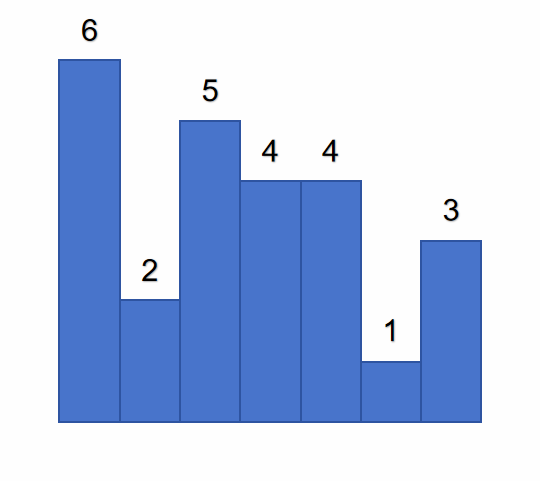
\includegraphics[width=6cm]{withnum.png}
        \caption{The Original Histogram}
    \end{minipage}
    \begin{minipage}[t]{0.48\textwidth}
        \centering
        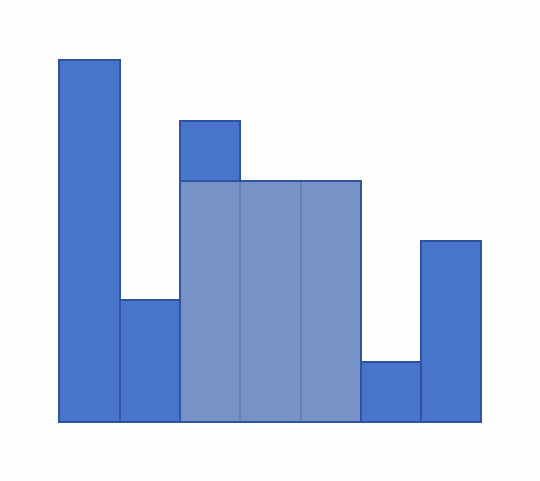
\includegraphics[width=6cm]{withrect.png}
        \caption{The Largest Rectangle in Histogram}
    \end{minipage}
\end{figure}

You may use $Rect(l, r, A)$ to represent the answer of the sub-problem w.r.t. the range $\left[l, r\right]$.

\begin{parts}
    \part[3] \textbf{Briefly} describe:
    \begin{enumerate}
        \item How would you divide the original problem into 2 sub-problems?
        \item Under what circumstances will the answer to the original problem not be covered by the answers of the 2 sub-problems?
        \item Given the answers of the 2 sub-problems, how would you get the answer of the original problem?
    \end{enumerate}
    
    \begin{solution}
    %%%%%%%%%%%%%%%%%%%%%%%%%%%%%%%%%%%%%%%%%%%%%%%%%
    % Replace `\vspace{2in}' with your answer.
    \\
    1.Find the shortest bar(or bars) in the histogram and set its index as smallestbar, and then calculate the maximum rectangular area of the two small histograms around the shortest bars by using Rect(l,smallestbar-1,A) and Rect(smallestbar+1,r,A).\\
    the sub-problem is calculating the largest rectangular area of the two part histograms around the shortest bars.\\
    2.When the area enclosed by the shortest bar(including the area enclosed by the left and right small histograms) is larger than the area of the largest rectangular area in the left and right small histograms, the answer to the original problem not be covered by the answers of the 2 sub-problems.\\
    3.Compare the area of the largest rectangle from the smallest histogram until the area of the larger of the two smaller histograms in the largest histogram is obtained, and compared with the area surrounded by the shortest bar, and then the larger one is the answer of the original problem.\\
    %%%%%%%%%%%%%%%%%%%%%%%%%%%%%%%%%%%%%%%%%%%%%%%%%
    \end{solution}

    \newpage
    
    \part[8] Based on your idea in part(a), design a \textbf{divide-and-conquer} algorithm for this problem. Make sure to provide \textbf{clear description} of your algorithm design in \textbf{natural language}, with \textbf{pseudocode} if necessary.
    
    \begin{solution}
    %%%%%%%%%%%%%%%%%%%%%%%%%%%%%%%%%%%%%%%%%%%%%%%%%
    % Replace `\vspace{7.5in}' with your answer.
    \\
    1.First, we traverse the histogram to find the shortest bar, then calculate the rectangular area surrounded by the shortest bar, and then operate the left and right histograms of the bar to find the largest rectangular area of each, and compare the larger one with the rectangle surrounded by the shortest bar to get the largest rectangular area.\\
    2.Similarly, to find the largest rectangular area of the two histograms, we first find the shortest bar, and then calculate the maximum rectangular area of its circumference, and the maximum rectangular area of the left and right histograms to find the maximum rectangular area between the three.\\
    3.This keeps dividing until the left and right histograms of the shortest bar contain only one bar.\\
    \\
    Pseudocode(maybe it does not satisfies the standard):\\
    \begin{cpp}
    left and right are indices of the left most and rightmost elements in given array arr respectively.\\
    function Rect(A, left, right)
        shortestbar = A[left];
        if right = left then
            return A[left]
        i = left;
        while(i < right)
            if (shortestbar > A[i++]) then
                shortestbar = A[i];
                shortestbarindex = i;
        if i = right then
            return max(shortestbar * (right-left+1), max(Rect(A, left, i-1), Rect(A, i+1, right)))
    \end{cpp}
    %%%%%%%%%%%%%%%%%%%%%%%%%%%%%%%%%%%%%%%%%%%%%%%%%
    \end{solution}

    \newpage
    
    \part[2] Provide the run-time complexity analysis of your algorithm in part (b). Make sure to include the \textbf{recurrence relation} of the run-time in your solution.
    
    \begin{solution}
    %%%%%%%%%%%%%%%%%%%%%%%%%%%%%%%%%%%%%%%%%%%%%%%%%
    % Replace `\vspace{3in}' with your answer.
    \\
    For the average case is that each sub-histogram can be divided constantly and be divided int a bar at the same level.\\
    On the zero level, we traverse the histogram and find the smallest bar which spend $\theta(n)$ time. And calculating the rectangle surrounded by the smallest bar and comparing the left and right indices spends constant time.\\
    And then we recursively divide the histogram into two smaller histograms by the smallest bar.\\
    For each smaller histogram, we spend the same proportion of time as the length of this histogram over the length of the larger histogram to traverse but all the total length of all histograms is approxiately the length of the histogram before it was divided.So on the next level, we spend the same time as before on the searching for the smallest bar. i.e. the work on the following level(all) is $\theta(n)$.\\
    Then for the average case, we get the recursive tree is that:\\
    Which recursive function is $T(n) = aT(\frac{n}{b}) + \theta(n)$ where a and b can be approximated as 2(for average).\\
    branching factor a,    the problem size is $\frac{n}{b^{k}}$ on the kth level and the work is $a^{k}(\frac{n}{b}^{k})^{d=1} = n$,  the levels is $logn$.\\
    Then the total time complexity of the algorithm is $\sum_{1}^{logn}a^{k}(\frac{n}{b^{k}}) = nlogn$.\\
    i.e. O(nlog(n))\\
    \\
    \\
    of course, if the histogram is an ascending or descending order, we can't divide it equally but one by one, then it's the worst case that we should do $\sum_{i=1}^{n}i$ = $\frac{n^{2}-n}{2}$ whose time complexity is $O(n^{2})$
    %%%%%%%%%%%%%%%%%%%%%%%%%%%%%%%%%%%%%%%%%%%%%%%%%
    \end{solution}
    
\end{parts}

\newpage

\titledquestion{Dividing with Creativity}

In this question, you are required analyze the run-time of algorithms with different dividing methods mentioned below. For each subpart except the third one, your answer should include:
\begin{enumerate}
    \item Describing the recurrence relation of the run-time $T(n)$. (Worth 1 point in 4)
    \item Finding the asymptotic order of the growth of $T(n)$ i.e. find a function $g$ such that $T(n) = O(g(n))$. Make sure your upper bound for $T(n)$ is tight enough. (Worth 1 point in 4)
    \item Show your \textbf{reasoning} for the upper bound of $T(n)$ or your process of obtaining the upper bound starting from the recurrence relation step by step. (Worth 2 points in 4)
\end{enumerate}

In each subpart, you may ignore any issue arising from whether a number is an integer as well as assuming \(T(0) = 0\) and \(T(1) = 1\). You can make use of the Master Theorem, Recursion Tree or other reasonable approaches to solve the following recurrence relations.

\begin{parts}
    \part[4] An algorithm $\mathcal{A}_1$ takes $\Theta(n)$ time to partition the original problem into 2 sub-problems, one of size $\lambda n$ and the other of size $(1-\lambda)n$ (here $\lambda \in \left(0, \frac{1}{2}\right)$), then recursively runs itself on both of the 2 sub-problems and finally takes $\Theta(n)$ time to merge the answers of the 2 sub-problems.
    
    \begin{solution}
    %%%%%%%%%%%%%%%%%%%%%%%%%%%%%%%%%%%%%%%%%%%%%%%%%
    % Replace `\vspace{5in}' with your answer.
    \\
    1.T(n) = T($\lambda$n) + T($(1-\lambda)n$) + $\theta(n)$\\
    2.T(n) = $O$(nlogn)\\
    3.Reason:\\
        because $A_{1}$ takes $\theta(n)$ time to partition the original problem into 2 sub-problem, and the size is $\lambda$ and $1-\lambda$ then the sub-problem naturally takes $\theta(\lambda(n))$, $\theta((1-\lambda)n)$. To ensure on the kth level, all the sub-pronblem is solved on constant time, (because $\lambda$ < $\frac{1}{2}$)then $(1 - \lambda)^{k} = \frac{1}{n}$ i.e.$k = log_{1-\lambda}(\frac{1}{n})$.\\
        So the zero level is n, then the 1th level is $\lambda(n)$, $(1-\lambda)n$, the 2nd level is $\lambda^{2}(n)$, $\lambda(1-\lambda)n$, $(1-\lambda)^{2}n$ ... So the total work T(n) = $\sum_{i=0}^{log_{1-\lambda}\frac{1}{n}}\sum_{j=0}^{i}C_{i}^{j}\lambda^{j}(1-\lambda)^{i-j}n$ = $\sum_{i=0}^{log_{1-\lambda}\frac{1}{n}}n = nlog_{1-\lambda}\frac{1}{n}$ and $\lambda \in (0, \frac{1}{2})$\\
        Therefore, the result  of T(n) is $O$(nlogn)\\
    %%%%%%%%%%%%%%%%%%%%%%%%%%%%%%%%%%%%%%%%%%%%%%%%%    
    \end{solution}

    \newpage
    
    \part[4] An algorithm $\mathcal{A}_2$ takes $\Theta(n)$ time to partition the original problem into 2 sub-problems, one of size $k$ and the other of size $(n - k)$ (here $k \in \mathbb{Z}^+$ is a constant), then recursively runs itself on both of the 2 sub-problems and finally takes $\Theta(n)$ time to merge the answers of the 2 sub-problems.
    
    \begin{solution}\\
    %%%%%%%%%%%%%%%%%%%%%%%%%%%%%%%%%%%%%%%%%%%%%%%%%
    % Replace `\vspace{1.5in}' with your answer.
    1.T(n) = T(n-k) + T(k) + $\theta(n)$\\
    2.T(n) = $\theta$($n^{2}$)\\
    3.from the zero level, to the 1st level, because one of size k and the other of size(n-k) and k is a constant, then the k size sub-problem can be solved in consant time which is $\theta(1)$ and don't need to partition next(since it has been solved).\\
    Then according to recursive tree, the size n-k sub-problem will be partitioned into size k and size n-2k with $\theta(n-k)$ time, and repeat the process above.\\
    Then we get the following series T(n) = n + $\theta(1)$ + n-k + $\theta(1)$ + n-2k + $\theta(1)$ + ... = $\frac{(n+k)*\frac{n}{k}}{2}$. Since k is a constant.\\
    Therefore, T(n) = $\theta(n^{2})$.
    %%%%%%%%%%%%%%%%%%%%%%%%%%%%%%%%%%%%%%%%%%%%%%%%%    
    \end{solution}

    \part{} Solve the recurrence relation $T(n) = T(\alpha n) + T(\beta n) + \Theta(n)$ where $\alpha + \beta < 1$ and $\alpha \geq \beta$.
    \begin{subparts}
        \subpart[2] Fill in the \textbf{four} blanks in the mathematical derivation snippet below.
        \begin{align*}
            T(n) &= T(\alpha n) + T(\beta n) + \Theta(n) \\
                 &= (T(\alpha ^2 n) + T(\alpha \beta n) + \Theta(\alpha n)) +
                    (T(\alpha \beta n) + T(\beta ^2 n) + \Theta(\beta n)) + \Theta(n) \\
                 &= (T(\alpha ^2 n) + 2T(\alpha \beta n) + T(\beta ^2 n)) + \Theta(n) (1 + (\alpha + \beta)) \\
                 &= \dots \\
                 &= \sum _ {i=0} ^k {C_{k}^{i}} T({\alpha^{i} \beta^{k-i} n}) + \Theta(n) \sum _ {j = 0} ^{{k-1}} \sum _ {l = 0} ^{j} {C_{k-1}^{l}\alpha^{l} \beta^{k-1-l}}
        \end{align*}

        \subpart[3] Based on the previous part, complete this question.
        \begin{solution}
        %%%%%%%%%%%%%%%%%%%%%%%%%%%%%%%%%%%%%%%%%%%%%%%%%
        % Replace `\vspace{3in}' with your answer.
        Because T(n) = T($\alpha$n) + T($\beta$n) + $\theta(n)$, then the zero level is cn(c is a positive constant).\\
        The level 1 is c$\alpha n$ and c$\beta n$.\\
        The level 2 is c$\alpha^{2} n$ c$\alpha \beta n$ c$\alpha \beta n$ c$\beta^{2} n$.\\
        and so on\\
        Then we get the following series\\
        T(n) = $c(n + (\alpha + \beta)n + (\alpha + \beta)^{2}n + ... + ) = cn(\frac{1}{1-(\alpha + \beta)})$ because $\alpha + \beta < 1$.\\
        Therefore, T(n) = $\theta(n)$.
        %%%%%%%%%%%%%%%%%%%%%%%%%%%%%%%%%%%%%%%%%%%%%%%%%
        \end{solution}
    \end{subparts}

    \newpage
    
    \part[4] An algorithm $\mathcal{A}_3$ takes $\Theta(\log n)$ time to convert the original problem into 2 sub-problems, each one of size $\sqrt{n}$, then recursively runs itself on both of the 2 sub-problems and finally takes $\Theta(\log n)$ time to merge the answers of the 2 sub-problems.
    
    Hint: W.L.O.G., you may assume $n = 2^m$ for $m \in \mathbb{Z}$.
    \begin{solution}
    %%%%%%%%%%%%%%%%%%%%%%%%%%%%%%%%%%%%%%%%%%%%%%%%%
    % Replace `\vspace{3in}' with your answer.
    1.T(n) = 2T($\sqrt{n}$) + $\theta(logn)$\\
    2.T(n) = O(lognloglogn)\\
    assume n = $2^{m}$ and it is transfromed to $A_{3}$ takes $\theta(m)$ time to convert the original problem into 2 sub-problems, each one of size $2^{\frac{m}{2}}$\\
    So T(n) is naturally transfromed into that $T(2^{m}) = T(2^{\frac{m}{2}}) + \theta(m)$.\\
    Then it equals the recursive tree that branching factor is 2, sub-problem size $\frac{n}{b}$ is $\frac{n}{2}$, the number of level is $log_{2}m$, so we get the series that T($2^{m}$) = $m + 2 * \frac{m}{2} + 2^{2} * (\frac{m}{2^{2}}) + ... + m*1 = m*log_{2}m$\\
    While n = $2^{m}$, then m = logn.\\
    i.e. T(n) = O(lognloglogn).
    %%%%%%%%%%%%%%%%%%%%%%%%%%%%%%%%%%%%%%%%%%%%%%%%%    
    \end{solution}
\end{parts}

\end{questions}

\end{document}